\subsection{Design method} \label{design_method}
We use Ampersand's method in this study.
The Ampersand method is based on relation algebra.
Ampersand makes it possible to create a Conceptual analysis of the source text. 
The conceptual and technical data model created with the descriptions in the Conceptual analysis allows the implementation to be based on it.

\subsubsection{Relation Algebra} \label{relation_algebra}
The field of relational algebra focuses on operations on sets.
The characteristic item of relation algebra is the relation.
This relation has its attributes.
The attributes in the example of \acrshort{big} would be the person's name, first names, gender, date of birth, nationality, and address, as well as the number and time of enrollment~\footnote{\acrlong{big} article 3, paragraph 2}.
The relation consists of tuples.
Since the relationship is always between two objects, one speaks of 2-tuples.
The tuples contain the attributes of the relation.

\begin{samepage}The operations on sets are the following:
\begin{itemize}
    \item Union, $R \cup S$ %vereniging
    \item Intersection, $R \cap S$ %doorsnede
    \item Difference, $R - S$ or $S - R$ %verschil
\end{itemize}
\end{samepage}
A distinction must be made between relation algebra~\citep{maddux_bibliography_2006} and relational algebra~\citep{codd_relational_1970}.
Ampersand uses relation algebra, so it is tuple related.
The relational algebra is the basis of e.g. relational databases which includes projections, selections and joins.
The latter are therefore not part of relation algebra.


\subsubsection{Ampersand} \label{ampersand}
Ampersand is based on relation algebra and focuses on business rules~\citepNonPub{wedemeijer_l_joosten_smm_michels_garkenbout_jlc_werkboek_ontwerpen_met_bedrijfsregelspdf_nodate}.
It supplies correct information systems.
Our goal is to use it to create a correct and error-free registration system.
Ampersand's other strengths are its support for conceptual analysis.
It is a platform for reactive programming and generates prototypes.
Ampersand script describes the goals rather than the steps.

Business rules are there to pursue a common goal.
These rules are converted to an information system using the Ampersand method.
The Ampersand method ensures that when a precise set of rules has been established, an information system can be generated.
To learn how Ampersand works in real life, we design a registry in Ampersand that implements the \acrshort{big}~\citepNonPub{van_wet_2018} .

\begin{wrapfigure} {r}{0.52\textwidth} 
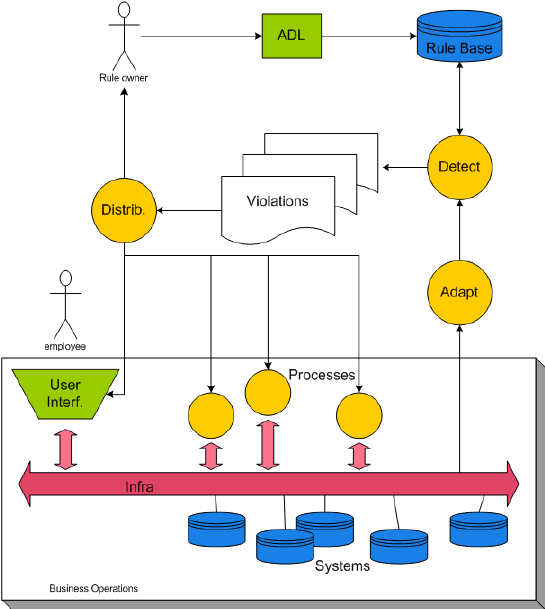
\includegraphics[width=7cm, height=6cm]{Principle-of-rule-based-process-management.png}
\caption{rule-based-proces}
\label{fig:rule-based-proces}
\end{wrapfigure}


The principle of rule-based \acrfull{bpm} as mentioned in \citepNonPub{joosten_joosten} is that any violation of a business rule may be used to trigger actions. 
This is described in the section \nameref{reactive_approach}.

Ampersand consists of concepts that in turn consist of atoms.
An atom is an implementation of the concept.
Inside the \acrshort{big} is a concept $beroep$ with associated atoms like $arts$, $tandarts$, etc" see listing~\ref{list:beroepen}.
We give the concepts a name so that the Concepts are recognized by the company.
This also applies to the definition and purpose of the terms.
These attributes are not mandatory, but when one wants to generate a functional design, these descriptions of the attributes are very useful.
\begin{lstlisting}[language=Octave, caption={Listing Concept Beroep},captionpos=b, label={list:beroepen}]
CONCEPT Beroep "Beroep van een persoon zoals bedoeld in de wet" 
PURPOSE CONCEPT Beroep 
{+Beroep dat uitgeoefend wordt+}
POPULATION Beroep CONTAINS [
    "arts",
    "tandarts",
    "apotheker",
    "gezondheidszorgpsycholoog",
    "psychotherapeut",
    "fysiotherapeut",
    "verloskundige",
    "verpleegkundige",
    "physician assistant",
    "orthopedagoog-generalist"
]
\end{lstlisting}

Concepts can have relationships with each other.
If the data of the concepts is true and the rules yield consistent data, then the relationships between real data are facts.
These facts together form one truth.
Not all concepts are directly related.
Within the domain of the \acrshort{big} we could distinguish the concept $registratie$ and the concept $beroep$.
These terms come from ~\citeNonPub{van_wet_2018} in article 3 of \acrshort{big}.
Even the name of the relationship is mentioned in this article, which the legislator calls a practitioner.
The law requires that details of the $registratie$ be recorded, stating the corresponding profession.
In Ampersand this is modeled as follows.
On the one hand the $beroep$ and also the concept $registratie$, see listing~\ref{list:concept_registratie}.
\begin{lstlisting}[language=Octave, caption={Listing Concept Registratie },captionpos=b, label={list:concept_registratie}] 
    CONCEPT Registratie "De registratie van een persoon binnen het register" 
    PURPOSE CONCEPT Registratie 
    {+Vastlegging in het register geeft toegang tot uitoefenen taak binnen de gezondheidszorg+}
\end{lstlisting}
Between the $registratie$ and the $persoon$ exists the relationship $beroepsbeoefenaar$, see listing~\ref{list:relatie_beroepsbeoefenaar}.
\begin{lstlisting}[language=Octave, caption={Listing RELATION "beroepsbeoefenaar" },captionpos=b, label={list:relatie_beroepsbeoefenaar}] 
RELATION beroepsbeoefenaar [Persoon*Registratie] 
MEANING "geregistreerd persoon"
POPULATION beroepsbeoefenaar CONTAINS 
[
  ("Piet",1);
  ("Susan",2);
  ("Gerard",3);
  ("John",4)
]\end{lstlisting}
By adding the concepts of $persoon$ (see listing~\ref{list:concept_persoon}) and $handeling$ (see listing~\ref{list:concept_handeling}), people may perform  medical actions, but only when they are qualified.
\begin{lstlisting}[language=Octave, caption={Listing Concept Persoon },captionpos=b, label={list:concept_persoon}] 
    CONCEPT Persoon "Persoon die werkzaam wilt zijn binnen de zorg"
    PURPOSE CONCEPT Persoon 
    {+Vastleggen van de identiteit van de persoon+}
\end{lstlisting}
\begin{lstlisting}[language=Octave, caption={Listing Concept Handeling },captionpos=b, label={list:concept_handeling}] 
    CONCEPT Handeling "Acties die uitgevoerd worden" 
    PURPOSE CONCEPT Handeling 
    {+Vastleggen van de mogelijke handelingen die uitgevoerd kunnen worden binnen de zorg+}
\end{lstlisting}
These concepts can lead us to the following scheme.
\begin{figure}[H] 
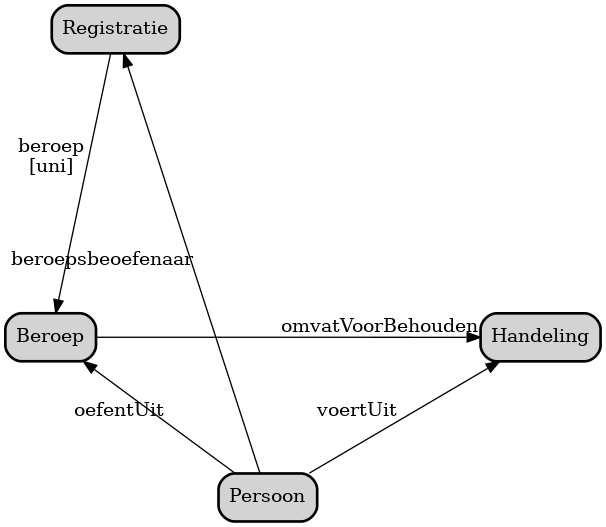
\includegraphics[scale=0.4]{CDConceptBeroep.png}
\centering
\caption{relations}
\label{fig:relations}
\end{figure}
The multiplicity must also be determined for each relation.
\begin{table}[h!]
    \caption{multiplicity}
    \begin{tabular}{||l | l||} 
     \hline
    function & The corresponding control question for the above relation $voerUit$ is\\
    \hline\hline
        Univalent & For each $Persoon$ there is at most one $Handeling$\\ %elke P max 1 H
        Total & For each $Persoon$ there is at least one $Handeling$ \\ %elke P minimaal 1 H
        Injective & For each $Handeling$ there is only one $Persoon$\\ %elke H max 1 P 
        Surjection & For each $Handeling$ there is at least one $Persoon$\\ %elke H minimaal 1 P
    \end{tabular}
    \label{tab:multiplicity}
\end{table}

Modeling using the Ampersand method determines which Concepts and Relationships arise within the research case.
Ampersand helps to gain insight into these connections.
This must be recognized by the analyst in the source text and defined in the script.
Ampersand then helps generate the functional design (the \acrshort{ca}) and the prototype.
Using the generated prototype, Ampersand validates the data with constraints on relationships.
This prevents registrations (data) that do not meet the requirements.
These restrictions are defined in rules within Ampersand (see for example list~\ref{list:rule_handelingdoorpersoon}).
A rule can be drawn up that determines whether a person is allowed to perform a certain action.
In figure \ref{fig:relations} the relations are named.
It was previously established that there are 2-tuple relationships.
Here we use the following notation:"$\mathit{relation [Concept \times Concept]}$".
\begin{center}
$\mathit{voertUit [Persoon \times Handeling]}$ ; 
 $\mathit{omvatVoorBehouden [Beroep \times Handeling]~\smallsmile}$
\newline $\subseteq$
\newline $\mathit{beroepsbeoefenaar [persoon \times registratie]}$ ;
$\mathit{beroep [registratie \times beroep]}$
\end{center}
The compared sets are
\newline $\mathit{[Persoon \times Beroep]}$
\newline The rule then will determine if the previous equation is true.
\newline If this is the case, then the rule is validated, otherwise the violation message occurs.
\begin{lstlisting} [language=Octave, caption={Listing Rule HandelingDoorPersoon },captionpos=b, label={list:rule_handelingdoorpersoon}] 
    RULE HandelingDoorPersoon: voertUit; omvatVoorBehouden[Beroep*Handeling]~ |- beroepsbeoefenaar; beroep
    MEANING "Een persoon mag handelingen uitvoeren wanneer hij een bepaald beroep uitoefend"
    MESSAGE "Geen toegestane handeling."
    VIOLATION (TXT "Persoon ", SRC I, TXT " voert de handeling uit ", TGT I, TXT " die niet tot zijn beroep behoren ", SRC I[Persoon];oefentUit)
\end{lstlisting}


\subsection{Reactive approach} \label{reactive_approach}
One of the benefits of Ampersand~\footnote{\url{https://ampersandtarski.gitbook.io/documentation/why-ampersand}} mentioned is the following statement "Use Ampersand as a platform for reactive programming, to help you of workflows and workflow models."

This reactive approach started with the reactive manifest~\citepNonPub{reactive_manifesto}.
The approach  defines the requirements that a reactive system should meet.
These include Responsive, Resilient, Elastic and Message Driven.
These requirements lead to systems that are flexible, loosely coupled and scalable, making them easier to develop and maintain.
Reactive Systems are made highly responsive and provide interactive feedback.
\begin{figure}[H] 
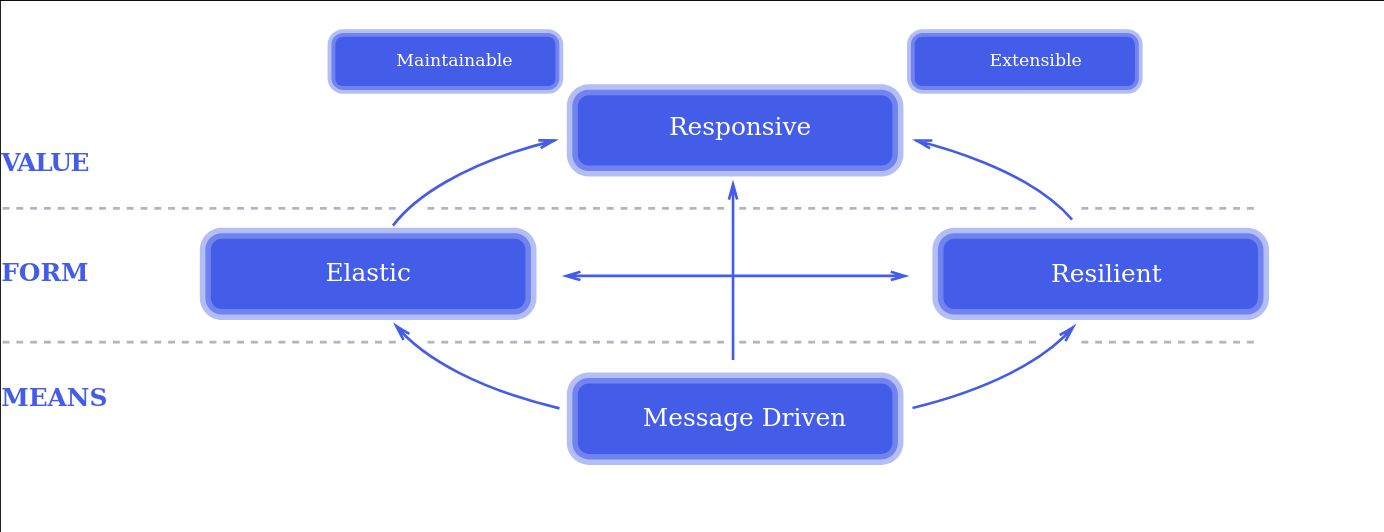
\includegraphics[scale=0.3]{reactive_manifesto.png}
\centering
\caption{reactive manifesto}
\label{fig:reactive manifesto}
\end{figure}

Ampersand is a form of Functional Reactive Programming (FRP)~\citep{elliott_functional_1997}.
The basic of reactive programming is the fact that it involves asynchronous communication.
The Reactive Manifest (see ~\citepNonPub{reactive_manifesto}) states that like uses message-driven systems, but Ampersand is more than a message-driven system.
This means that, as the Reactive Manifest prescribes, it uses message-driven systems, but Ampersand is more than a message-driven system.It is actually an event-driven system.
The glossary of the \citeNonPub{reactive_manifesto} indicates the difference between message driven systems and event driven systems.
An event-driven system targets event-bus while a message-driven system targets recipients~\citep{bainomugisha_survey_2013}.
The essence is that the order of the flow cannot be determined in advance.
The system will respond to events caused by constraints.
Ampersand determines the dynamic flow~\citep{joosten_relation_2018}.

